% Dados: metadados das respostas do Ollama nas execuções de 10/09, 15/09 e 19/10/2026 (29 planos cada)
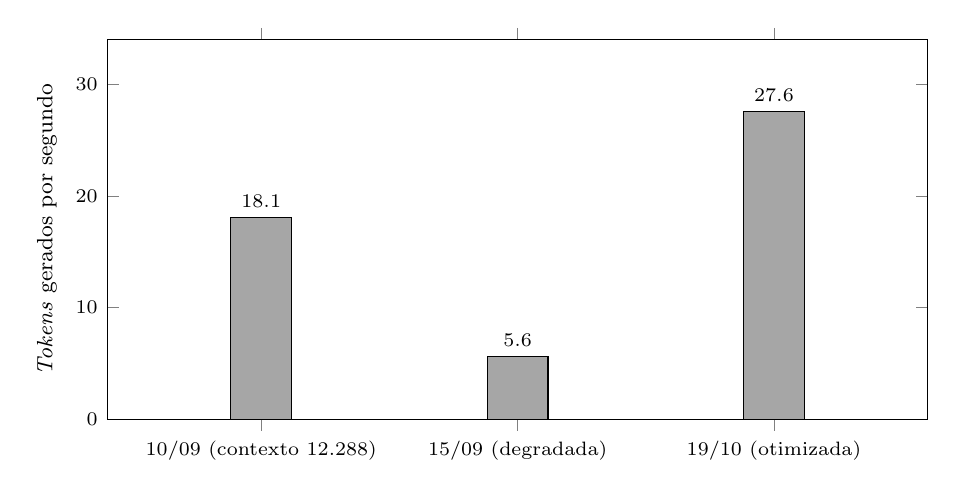
\begin{tikzpicture}
\begin{axis}[
  ybar,
  width=12cm, height=6.4cm,
  bar width=22pt,
  ymin=0, ymax=34,
  ylabel={\textit{Tokens} gerados por segundo},
  symbolic x coords={10/09,15/09,19/10},
  xtick=data,
  xticklabels={{10/09 (contexto 12.288)},{15/09 (degradada)},{19/10 (otimizada)}},
  nodes near coords={\pgfmathprintnumber[fixed,precision=1]{\pgfplotspointmeta}},
  nodes near coords style={font=\scriptsize},
  ticklabel style={font=\scriptsize},
  label style={font=\footnotesize},
  enlarge x limits=0.3,
]
\addplot[fill=black!35, draw=black] coordinates {(10/09,18.1) (15/09,5.6) (19/10,27.6)};
\end{axis}
\end{tikzpicture}
